% Created 2019-02-14 Thu 12:33
% Intended LaTeX compiler: pdflatex
\documentclass[a4paper, twoside, 12pt]{article}
\usepackage[utf8]{inputenc}
\usepackage[T1]{fontenc}
\usepackage{graphicx}
\usepackage{grffile}
\usepackage{longtable}
\usepackage{wrapfig}
\usepackage{rotating}
\usepackage[normalem]{ulem}
\usepackage{amsmath}
\usepackage{textcomp}
\usepackage{amssymb}
\usepackage{capt-of}
\usepackage{hyperref}
\usepackage[left=2.5cm, right=2.5cm, top=2.5cm, bottom=2.5cm, bindingoffset=1.5cm, head=15pt]{geometry}
\usepackage{setspace}
\usepackage{caption}
\onehalfspacing
\usepackage[official]{eurosym}
\usepackage{amsmath}
\usepackage{amssymb}
\usepackage{format/notation}
\usepackage{fancyhdr}
\pagestyle{fancy}
\fancyhead{}
\fancyfoot{}
\fancyhead[LE,RO]{\textsl{\leftmark}}
\fancyhead[RE,LO]{Tobias Richter}
\fancyfoot[C]{\thepage}
\renewcommand{\headrulewidth}{0.4pt}
\renewcommand{\footrulewidth}{0pt}
\usepackage{apacite}
\let\cite\shortcite
\let\textcite\shortciteA
\usepackage[nohyperlinks]{acronym}
\interfootnotelinepenalty=10000
\usepackage[notlof,notlot,nottoc]{tocbibind}
\newcommand{\studentID}{558305}
\newcommand{\thesistype}{Master Thesis}
\newcommand{\supervisor}{Univ.-Prof. Dr. Wolfgang Ketter}
\newcommand{\cosupervisor}{Karsten Schroer, Philipp Artur Kienscherf}
\pagenumbering{Roman}
\author{Tobias Richter}
\date{\today}
\title{Reinforcement Learning Portfolio Optimization of Electric Vehicle Virtual Power Plants}
\hypersetup{
 pdfauthor={Tobias Richter},
 pdftitle={Reinforcement Learning Portfolio Optimization of Electric Vehicle Virtual Power Plants},
 pdfkeywords={},
 pdfsubject={},
 pdfcreator={Emacs 26.1 (Org mode 9.2.1)},
 pdflang={English}}
\begin{document}

\makeatletter
\begin{titlepage}
    \begin{center}
        \vspace*{1cm}

        \Large
        \textbf{\@title{}}

        \vspace{1.5cm}

        \thesistype{}

        \vspace{1cm}

        \begin{figure}[htbp]
             \centering
             
\includegraphics[width=.5\linewidth]{./fig/UoC_Logo.png}
        \end{figure}

        \vspace{1cm}

        \large
        \textbf{Author}: \@author{} (Student ID: \studentID{})\\
        \large
        \textbf{Supervisor}: \supervisor{}\\
        \large
        \textbf{Co-Supervisor}: \cosupervisor{}

        \vspace{1cm}
        \large
        Department of Information Systems for Sustainable Society\\
        Faculty of Management, Economics and Social Sciences\\
        University of Cologne\\

        \vspace{1cm}
        \@date{}

    \end{center}
\end{titlepage}
\makeatother
\clearpage
\thispagestyle{empty}
\section*{Eidesstattliche Versicherung}
\label{sec:SOOA}

\vspace{2.5cm}

% Statement of original authorship - Needs to be in German
% see also here: https://www.wiso.uni-koeln.de/sites/fakultaet/dokumente/PA/formulare/eidesstattliche_erklaerung.pdf

Hiermit versichere ich an Eides statt, dass ich die vorliegende Arbeit selbstständig und ohne die Benutzung anderer als der angegebenen Hilfsmittel angefertigt habe. Alle Stellen, die wörtlich oder sinngemäß aus veröffentlichten und nicht veröffentlichten Schriften entnommen wurden, sind als solche kenntlich gemacht. Die Arbeit ist in gleicher oder ähnlicher Form oder auszugsweise im Rahmen einer anderen Prüfung noch nicht vorgelegt worden. Ich versichere, dass die eingereichte elektronische Fassung der eingereichten Druckfassung vollständig entspricht.

\vspace{1cm}

\noindent
Die Strafbarkeit einer falschen eidesstattlichen Versicherung ist mir bekannt, namentlich die Strafandrohung gemäß § 156 StGB bis zu drei Jahren Freiheitsstrafe oder Geldstrafe bei vorsätzlicher Begehung der Tat bzw. gemäß § 161 Abs. 1 StGB bis zu einem Jahr Freiheitsstrafe oder Geldstrafe bei fahrlässiger Begehung.

\vspace{3cm}
\noindent
\textbf{\@author{}}

\vspace{0.5cm}
\noindent
Köln, den xx.xx.20xx
\clearpage

\setcounter{page}{1}
\tableofcontents
\clearpage
\listoffigures
\clearpage
\listoftables
\clearpage

\section*{List of Abbreviations} \markboth{LIST OF ABBREVIATIONS}{}
\begin{acronym}[GCRM]
	\acro{ANN}{Artificial Neural Network}
	\acro{DSO}{Distribution System Operator}
	\acro{DP}{Dynamic Programming}
	\acro{EV}{Electric Vehicle}
	\acro{GP}{Genetic Programming}
	\acro{GPI}{Generalized Policy Iteration}
	\acro{GCRM}{German Control Reserve Market}
	\acro{MAW}{Mean Asymmetric Weighted Objective Function}
	\acro{MC}{Monte Carlo}
	\acro{MDP}{Markov Decision Process}
	\acro{PDF}{Probability Density Function}
	\acro{RL}{Reinforcement Learning}
	\acro{TD}{Temporal-Difference}
	\acro{V2G}{Vehicle-to-Grid}
	\acro{VPP}{Virtual Power Plant}
\end{acronym}
\clearpage
\section*{Summary of Notation} \markboth{SUMMARY OF NOTATION}{}
Capital letters are used for random variables, whereas lower case letters are used for
the values of random variables and for scalar functions. Quantities that are required to
be real-valued vectors are written in bold and in lower case (even if random variables).
\begin{tabbing}
    \=~~~~~~~~~~~~~~~~~~  \= \kill
    \>$\defeq$            \> equality relationship that is true by definition\\
    \>$\approx$           \> approximately equal\\
    % \>$\propto$           \> proportional to\\
    \>$\Pr{X\!=\!x}$      \> probability that a random variable $X$ takes on the value $x$\\
    % \>$X\sim p$           \> random variable $X$ selected from distribution $p(x)\defeq\Pr{X\!=\!x}$\\
    \>$\E{X}$             \> expectation of a random variable $X$, i.e., $\E{X}\defeq\sum_x p(x)x$\\
    % \>$\arg\max_a f(a)$   \> a value of $a$ at which $f(a)$ takes its maximal value\\
    % \>$\ln x$             \> natural logarithm of $x$\\
    % \>$e^x$               \> the base of the natural logarithm, $e\approx 2.71828$, carried to power $x$; $e^{\ln x}=x$\\
    \>$\Re$               \> set of real numbers\\
    % \>$f:\X\rightarrow\Y$ \> function $f$ from elements of set $\X$ to elements of set $\Y$\\
    \>$\leftarrow$        \> assignment\\
    % \>$(a,b]$             \> the real interval between $a$ and $b$ including $b$ but not including $a$\\
    \\
    \>$\e$                \> probability of taking a random action in an \e-greedy policy\\
    \>$\alpha, \beta$     \> step-size parameters\\
    \>$\gamma$            \> discount-rate parameter\\
    % \>$\lambda$           \> decay-rate parameter for eligibility traces\\
    % \>$\ind{\text{\emph{predicate}}}$ \>indicator function ($\ind{\text{\emph{predicate}}}\defeq1$ if the \emph{predicate} is true, else 0)\\
    \\
    \>$s, s'$             \> states\\
    \>$a$                 \> an action\\
    \>$r$                 \> a reward\\
    \>$\S$                \> set of all nonterminal states \\
    % \>$\S^+$              \> set of all states, including the terminal state \\
    \>$\A$                \> set of all available actions\\
    \>$\R$                \> set of all possible rewards, a finite subset of $\Re$\\
    \>$\subset$           \> subset of; e.g., $\R\subset\Re$\\
    \>$\in$               \> is an element of; e.g., $s\in\S$, $r\in\R$\\
    % \>$|\S|$              \> number of elements in set $\S$\\
    \\
    \>$t$                 \> discrete time step\\
    \>$T, T(t)$           \> final time step of an episode, or of the episode including time step $t$\\
    \>$A_t$               \> action at time $t$\\
    \>$S_t$               \> state at time $t$, typically due, stochastically, to $S_{t-1}$ and $A_{t-1}$\\
    \>$R_t$               \> reward at time $t$, typically due, stochastically, to $S_{t-1}$ and $A_{t-1}$\\
    \>$\pi$               \> policy (decision-making rule)\\
    \>$\pi(s)$            \> action taken in state $s$ under {\it deterministic\/} policy $\pi$\\
    \>$\pi(a|s)$          \> probability of taking action $a$ in state $s$ under {\it stochastic\/} policy $\pi$\\
    \\
    \>$G_t$               \> return following time $t$\\
    % \>$h$                 \> horizon, the time step one looks up to in a forward view\\
    % \>$G_{t:t+n}, G_{t:h}$\> $n$-step return from $t+1$ to $t+n$, or to $h$ (discounted and corrected) \\
    % \>$\bar G_{t:h}$      \> flat return (undiscounted and uncorrected) from $t+1$ to $h$\\
    % \>$G^\lambda_t$       \> $\lambda$-return\\
    % \>$G^\lambda_{t:h}$   \> truncated, corrected $\lambda$-return\\
    % \>$G^{\lambda s}_t$, $G^{\lambda a}_t$    \> $\lambda$-return, corrected by estimated state, or action, values \\
    % \\
    \>$\p(s',r|s,a)$      \> probability of transition to state $s'$ with reward $r$, from state $s$ and action $a$\\
    \>$\p(s'|s,a)$        \> probability of transition to state $s'$, from state $s$ taking action $a$\\
    % \>$r(s,a)$            \> expected immediate reward from state $s$ after action $a$\\
    % \>$r(s,a,s')$         \> expected immediate reward on transition from $s$ to $s'$ under action $a$\\
    % \\
    \>$\vpi(s)$           \> value of state $s$ under policy $\pi$ (expected return)\\
    \>$\vstar(s)$         \> value of state $s$ under the optimal policy \\
    \>$\qpi(s,a)$         \> value of taking action $a$ in state $s$ under policy $\pi$\\
    \>$\qstar(s,a)$       \> value of taking action $a$ in state $s$ under the optimal policy \\
    % \\
    \>$V, V_t$            \> array estimates of state-value function $\vpi$ or $\vstar$\\
    \>$Q, Q_t$            \> array estimates of action-value function $\qpi$ or $\qstar$\\
    % \>$\bar V_t(s)$       \> expected approximate action value, e.g., $\bar V_t(s)\defeq\sum_a\pi(a|s)Q_{t}(s,a)$\\
    % \>$U_t$               \> target for estimate at time $t$\\
    % \\
    % \>$\delta_t$          \> temporal-difference (TD) error at $t$ (a random variable) \\
    % \>$\delta^s_t, \delta^a_t$ \> state- and action-specific forms of the TD error \\
    % \>$n$                 \> in $n$-step methods, $n$ is the number of steps of bootstrapping\\
    % \\
    \>$d$                 \> dimensionality---the number of components of $\w$\\
    % \>$d'$                \> alternate dimensionality---the number of components of $\th$\\
    \>$\w$           \> $d$-vector of weights underlying an approximate value function\\
    % \>$w_i,w_{t,i}$ \> $i$th component of learnable weight vector\\
    \>$\hat v(s,\w)$      \> approximate value of state $s$ given weight vector $\w$\\
    % \>$v_\w(s)$           \> alternate notation for $\hat v(s,\w)$\\
    % \>$\hat q(s,a,\w)$    \> approximate value of state--action pair $s,a$ given weight vector $\w$\\
    % \>$\grad \hat v(s,\w)$\> column vector of partial derivatives of $\hat v(s,\w)$ with respect to $\w$\\
    % \>$\grad \hat q(s,a,\w)$\> column vector of partial derivatives of $\hat q(s,a,\w)$ with respect to $\w$\\
    % \\
    % \>$\x(s)$             \> vector of features visible when in state $s$\\
    % \>$\x(s,a)$           \> vector of features visible when in state $s$ taking action $a$\\
    % \>$x_i(s), x_i(s,a)$  \> $i$th component of vector $\x(s)$ or $\x(s, a)$\\
    % \>$\x_t$              \> shorthand for $\x(S_t)$ or $\x(S_t,A_t)$\\
    % \>$\w\tr\x$           \> inner product of vectors, $\w\tr\x\defeq\sum_i w_i x_i$; e.g., $\hat v(s,\w)\defeq\w\tr\x(s)$\\
    % \>$\v,\v_t$           \> secondary $d$-vector of weights, used to learn $\w$ \\
    % \>$\z_t$              \> $d$-vector of eligibility traces at time $t$ \\
    % \\
    % \>$\th, \th_t$        \> parameter vector of target policy \\
    % \>$\pi(a|s,\th)$      \> probability of taking action $a$ in state $s$ given parameter vector $\th$\\
    % \>$\pi_\th$           \> policy corresponding to parameter $\th$\\
    % \>$\grad\pi(a|s,\th)$ \>column vector of partial derivatives of $\pi(a|s,\th)$ with respect to $\th$\\
    % \>$J(\th)$            \> performance measure for the policy $\pi_\th$\\
    % \>$\grad J(\th)$      \> column vector of partial derivatives of $J(\th)$ with respect to $\th$\\
    % \>$h(s,a,\th)$        \> preference for selecting action $a$ in state $s$ based on $\th$\\
    % \\
    % \>$b(a|s)$            \> behavior policy used to select actions while learning about target policy $\pi$ \\
    % \>$b(s)$              \> a baseline function $b:\S\mapsto\Re$ for policy-gradient methods\\
    % \>$b$                 \> branching factor for an MDP or search tree \\
    % \>$\rho_{t:h}$        \> importance sampling ratio for time $t$ through time $h$ \\
    % \>$\rho_{t}$          \> importance sampling ratio for time $t$ alone, $\rho_t\defeq\rho_{t:t}$\\
    % \>$r(\pi)$            \> average reward (reward rate) for policy $\pi$ \\
    % \>$\bar R_t$          \> estimate of $r(\pi)$ at time $t$\\
    % \\
    % \>$\mu(s)$            \> on-policy distribution over states \\
    % \>$\bm\mu$            \> $|\S|$-vector of the $\mu(s)$ for all $s\in\S$\\
    % \>$\norm{v}$          \> $\mu$-weighted squared norm of value function $v$, i.e., $\norm{v}\defeq\sum_{s\in\S} \mu(s)v(s)^2$\\
    % \>$\eta(s)$           \> expected number of visits to state $s$ per episode\\
    % \>$\Pi$               \> projection operator for value functions \\
    % \>$B_\pi$             \> Bellman operator for value functions \\
    % \\
    % \>${\bf A}$           \> $d\times d$ matrix ${\bf A}\defeq\E{\x_t\bigl(\x_t-\g\x_{t+1}\bigr)\tr}$\\
    % \>${\bf b}$           \> $d$-dimensional vector ${\bf b}\defeq\E{R_{t+1}\x_t}$\\
    % \>$\w_{\rm TD}$       \> TD fixed point $\w_{\rm TD}\defeq {\bf A}^{-1}{\bf b}$ (a $d$-vector\\
    % \>${\bf I}$           \> identity matrix\\
    % \>${\bf P}$           \> $|\S|\times |\S|$ matrix of state-transition probabilities under $\pi$\\
    % \>${\bf D}$           \> $|\S|\times |\S|$ diagonal matrix with $\bm\mu$ on its diagonal\\
    % \>${\bf X}$           \> $|\S|\times d$ matrix with the $\x(s)$ as its rows\\
    % \\
    % \>$\bar\delta_\w(s)$  \> Bellman error (expected TD error) for $v_\w$ at state $s$\\
    % \>$\bar\delta_\w$, BE \> Bellman error vector, with components $\bar\delta_\w(s)$\\
    \>$\MSVEm(\w)$        \> mean square value error $\MSVEm(\w)\defeq\norm{v_\w-\vpi}$\\
    % \>$\MSBEm(\w)$        \> mean square Bellman error $\MSBEm(\w)\defeq\norm{\bar\delta_\w}$\\
    % \>$\MSPBEm(\w)$       \> mean square projected Bellman error $\MSPBEm(\w)\defeq\norm{\Pi\bar\delta_\w}$\\
    % \>$\MSTDEm(\w)$       \> mean square temporal-difference error $\MSTDEm(\w)\defeq\EE{b}{\rho_t\delta_t^2}$ \\
    % \>$\MSREm(\w)$        \> mean square return error\\
\end{tabbing}
\clearpage

\pagenumbering{arabic}

\section{Introduction (10\%)}
\label{sec:org5911709}
\subsection{Research Motivation}
\label{sec:orgedb51aa}
\begin{itemize}
\item \cite{lopes11_integ_elect_vehic_elect_power_system}
\end{itemize}
\subsection{Research Question}
\label{sec:orgfbb6e9b}
\subsection{Relevance}
\label{sec:org3532569}

\clearpage
\section{Related Literature (10\%)}
\label{sec:org1f9bbac}
\subsection{Smart Charging and Balancing the Electric Grid with EV Fleets}
\label{sec:org1e10e2a}
The increasing penetration of EVs has a substantial effect on electricity
consumption patterns. During charging periods, power flows and grid losses
increase considerably and challenge the grid. Operators have to reinforce the
grid to ensure that transformers and substations do not overload
\cite{sioshansi12_impac_elect_tarif_plug_in,lopes11_integ_elect_vehic_elect_power_system}.
Loading multiple EVs in the same neighborhood, or worse, whole EV fleets at
once, stress the grid. In these cases, even brown- or blackouts can occur.
\cite{kim12_carbit}. Despite these challenges, it is possible to support the
physical reinforcement by adopting smart charging strategies. In smart charging,
EVs get charged when the grid is less congested to ensure grid stability. Smart
charging reduces peaks in electricity demand, called \emph{Peak Cutting}, and
complement the grid in times of low demand, called \emph{Valley Filling}. Smart
charging has been researched thoroughly in the IS literature, in the following
we will outline some of the most important contributions.


\textcite{valogianni14_effec_manag_elect_vehic_storag} found that using
intelligent agents to schedule EV charging substantially reshapes the energy
demand and reduces peak demand without violating individual household
preferences. Moreover, they showed that the proposed smart charging behavior
reduces average energy prices and thus benefit households economically. In
another study, \textcite{kara15_estim_benef_elect_vehic_smart} investigated the
effect of smart charging on public charging stations in California. Controlling
for arrival and departure times, the authors presented beneficial results for
the distribution system operator (DSO) and the owners of EVs. Their approach
resulted in a price reduction in energy bills and a peak load reduction. An
extension of the smart charging concept is Vehicle-to-Grid (V2G). When equipped
with V2G devices, EVs can discharge their batteries back into the grid. Existing
research has focused on this technology in respect to grid stabilization effects
and arbitrage possibilities. For instance,
\textcite{schill11_elect_vehic_imper_elect_market} showed that the usage of EVs
can decrease average consumer electricity prices. Excess EV battery capacity can
be used to charge in off-peak hours and discharge in peak hours, when the prices
are higher. These arbitrage possibilities reverse welfare effects of generators
and increase the overall welfare and consumer surplus.
\textcite{tomic07_using_fleet_elect_drive_vehic_grid_suppor} found that the
arbitrage opportunities are especially prominent when a high variability in
electricity prices on the target electricity market exists. The authors stated
that short intervals between the contract of sale and the physical delivery of
electricity increase arbitrage benefits. Consequently, ancillary service
markets, like frequency control and operating reserve markets, are attractive
for smart charging.

\textcite{peterson10_econom_using_plug_in_hybrid} investigated energy arbitrage
profitability with V2G in the light of battery depreciation effects in the US.
The results of their study indicate that large-scale use of EV batteries for
grid storage does not yield enough monetary benefits to incentivize EV owners to
participate in V2G activities. Considering battery depreciation cost, the
authors arrived at an annual profit of only 6\$ - 72\$ per EV.
\textcite{brandt17_evaluat_busin_model_vehic_grid_integ} evaluated a business
model for parking garage operators operating on the German frequency regulation
market. When taking infrastructure costs and battery depreciation costs into
account, they conclude that the proposed vehicle-grid integration is not
profitable. Even with generous assumptions about EV adoption rates in Germany
and altered auction mechanisms, the authors arrived at negative profits.
\textcite{kahlen17_fleet} used EV fleets to offer balancing services to the grid.
Evaluating the impact of V2G in their model, the authors conclude that V2G would
only be profitable if reserve power prices were twice as high. Considering the
results from the studies mentioned above, our research does not include V2G,
since only marginal profits are expected.

In order to maximize profits, it is essential for market participants to develop
successful bidding strategies. Several authors have investigated bidding
strategies to jointly participate in multiple markets
\cite{mashhour11_biddin_strat_virtual_power_plant_2,he16_optim_biddin_strat_batter_storag}.
\textcite{mashhour11_biddin_strat_virtual_power_plant_2} used stationary battery
storage to participate in the spinning reserve market and the day-ahead market
at the same time. The authors developed a non-equilibrium model, which solves
the presented mixed-integer program with Genetic Programming (GP). Contrarily,
we use a model-free RL agent that learns an optimal policy (i.e., a trading
strategy) from actions it takes in the environment (i.e., bidding on electricity
markets). Using a model-free approach is especially beneficial for us, since
additional unknown variables and constraints (i.e., customer mobility demand)
complicate the formulation of a mathematical model.

\textcite{he16_optim_biddin_strat_batter_storag} conducted similar research to
\textcite{mashhour11_biddin_strat_virtual_power_plant_2}. The authors additionally
incorporated battery life cycle in their profit maximization model, which proved
to be a decisive factor. In contrast to the authors, we jointly participated in
the secondary operating reserve and spot market with the \emph{non-stationary}
storage of EV batteries. Because shared EVs have to satisfy mobility demand,
they have to be charged in any case, which allows us to safely exclude battery
depreciation from our model. Further, we chose the intraday market over the
day-ahead market, as it has the lowest reaction time among the spot markets, and
thus potentially offers higher profits
\cite{tomic07_using_fleet_elect_drive_vehic_grid_suppor}.

Previous studies often assume that car owners or households can directly trade
on electricity markets. In reality, this is not possible due to the minimum
capacity requirements of the markets, requirements that single EVs do not meet.
For example, the German Control Reserve Market (GCRM) has a minimum trading
capacity of 1MW to 5MW, depending on the specific market. In order to reach the
minimum capacity, over 200 EVs would need to be connected to the grid via a
standard 4.6kW charging station at the same time. \textcite{ketter13_power_tac}
introduced the notion of electricity brokers, aggregators that act on behalf of
a group of individuals or households to participate in electricity markets.
\textcite{brandt17_evaluat_busin_model_vehic_grid_integ} and
\textcite{kahlen14_balan_with_elect_vehic} successfully showed that electricity
brokers can overcome the capacity issues by aggregating EV batteries. In
addition to electricity brokers, we apply the concept of Virtual Power Plants
(VPPs). VPPs are flexible portfolios of distributed energy resources, which are
presented with a single load profile to the system operator, making them
eligible for market participation and ancillary service provisioning
\cite{pudjianto07_virtual_power_plant_system_integ}. Hence, VPPs allow providing
regulation capacity to the market without knowing which exact sources provide
the promised capacity until the delivery time \cite{kahlen17_fleet}. This concept
is specially useful when dealing with EV fleets: VPPs enable carsharing
providers to issue bids and asks based on an estimate of available fleet
capacity, without knowing beforehand which exact EVs will provide the capacity
at the time of delivery. Based on the battery charge and the availability of
EVs, an intelligent agent decides in real-time which vehicles provide the
capacity.

Centrally managed EV fleets make it possible for carsharing providers to use the
presented concepts as a viable business extension. Free float carsharing is a
popular concept that allows cars to be picked up and parked everywhere, and the
customers are billed is by the minute. Free float carsharing offers flexibility
to its users, saves resources, and reduces carbon emissions
\cite{firnkorn15_free_float_elect_carsh_fleet_smart_cities}. Most previous studies
concerned with the usage of EVs for electricity trading, assumed that trips are
fixed and known in advance, e.g., in
\textcite{tomic07_using_fleet_elect_drive_vehic_grid_suppor}. The free float
concept adds uncertainty and nondeterministic behavior, which make predictions
about future rentals a complex issue.

\textcite{kahlen17_fleet} showed that it is possible to use free float carsharing
fleets as VPPs to profitably offer balancing services to the grid. In their
study, the authors compared cases from three different cities across Europe and
the US. They used an event-based simulation, bootstrapped with real-world
carsharing and secondary operating reserve market data from the respective
cities. A central dilemma within their research was to decide whether an EV
should be committed to a VPP or free for rent. Since rental profits are
considerably higher than profits from electricity trading, it is crucial not to
allocate an EV to a VPP when it could have been rented out otherwise. To deal
with the asymmetric payoff, \citeauthor{kahlen17_fleet} used stratified sampling
in their classifier. This method gives rental misclassifications higher weights,
reducing the likelihood of EVs to participate in VPP activities. The authors
used a Random Forest regression model to predict the available balancing
capacity on an aggregated fleet level. Only at the delivery time, the agent
decides which individual EVs provide the regulation capacity. This heuristic is
based on the likelihood that the vehicle is rented out and on its expected
rental benefits.

In a similar study, the authors showed that carsharing companies can participate
in day-ahead markets for arbitrage purposes
\cite{kahlen18_elect_vehic_virtual_power_plant_dilem}. In the paper, the authors
used a sinusoidal time-series model to predict the available trading capacity.
Another central problem for carsharing providers is that committed trades, which
can not be fulfilled, result in substantial penalties from the system operator
or electricity exchange. In other words, fleet operators have to avoid buying
any amount of electricity, which they can't be sure to charge with available EVs
at the delivery time. To address this issue, the authors developed a mean
asymmetric weighted (MAW) objective function. They used it for their time-series
based prediction model, to penalize committing an EV to VPP when it would have
been rented out otherwise. Because of the two issues mentioned above,
\textcite{kahlen18_elect_vehic_virtual_power_plant_dilem} could only make very
conservative estimations and commitments of overall available trading capacity,
resulting in a high amount of foregone profits. This effect is especially
prominent when participating in the secondary operating reserve market, since
commitments have to be made one week in advance when mobility demands are still
uncertain. \textcite{kahlen17_fleet} stated that in 42\% to 80\% of the cases, EVs
are \emph{not} committed to a VPP when it would have been profitable to do so.

This thesis proposes a solution in which the EV fleet participates in the
balancing market and intraday market simultaneously. With this approach, we
align the potentially higher profits on the balancing markets, with more
accurate capacity predictions for intraday markets
\cite{tomic07_using_fleet_elect_drive_vehic_grid_suppor}. This research followed
\textcite{kahlen17_fleet}, who proposed to work on a combination of multiple
markets in the future.

\subsection{Reinforcement Learning in Smart Grids}
\label{sec:org905bd81}

Previous research shows that intelligent agents equipped with Reinforcement
Learning (RL) methods can successfully take action in the smart grid. The
following chapter outlines different research approaches of RL in the domain of
smart grids. For a more thorough description, mathematical formulations and
common issues, of RL refer to Chapter \ref{sec-reinforcement-learning}.

\textcite{reddy11_learn_behav_multip_auton_agent,reddy11_strat} used autonomous
broker agents to buy and sell electricity from DER on a proposed \emph{Tariff
Market}. The agents use Markov Decision Processes (MDPs) and RL to learn pricing
strategies to profitably participate in the Tariff Market. To control for a
large number of possible states in the domain, the authors used \emph{Q-Learning}
with derived state space features. Based on descriptive statistics, they defined
derived price and market participant features. By engaging with its environment,
the agent learns an optional sequence of actions (policy) based on the state of
the agent. \textcite{peters13_reinf_learn_approac_to_auton} built on that work and
further enhanced the method by using function approximation. Function
approximation allows to efficiently learn strategies over large state spaces, by
deriving a function that describes the states instead of defining discrete
states. By using this technique, the agent can adapt to arbitrary economic
signals from its environment, resulting in better performance than previous
approaches. Moreover, the authors applied feature selection and regularization
methods to explore the agent's adaption to the environment. These methods are
particularly beneficial in smart markets because market design, structures, and
conditions might change in the future. Hence, intelligent agents should be able
to adapt to it \cite{peters13_reinf_learn_approac_to_auton}.

\textcite{vandael15_reinf_learn_heuris_ev_fleet} facilitated learned EV fleet
charging behavior to optimally purchase electricity on the day-ahead market.
Similarly to \textcite{kahlen18_elect_vehic_virtual_power_plant_dilem}, the problem
is framed from the viewpoint of an aggregator that tries to define a
cost-effective day-ahead charging plan in the absence of knowing EV charging
parameters, such as departure time. A crucial point of the study is weighting low
charging prices against costs that have to be paid when an excessive
or insufficient  amount of electricity is bought from the market (imbalance costs). Contrarily,
\textcite{kahlen18_elect_vehic_virtual_power_plant_dilem} did not consider
imbalance cost in their model and avoid them by sacrificing customer mobility in order
to balance the market (i.e., not showing the EV available for rent, when it is
providing balancing capacity). \textcite{vandael15_reinf_learn_heuris_ev_fleet}
used a \emph{fitted Q Iteration} to control for continuous variables in their state and
action space. In order to achieve fast convergence, they additionally optimized
the \emph{temperature step} parameter of the Boltzmann exploration probability.


\textcite{dusparic13_multi} proposed a multi-agent approach for residential demand
response. The authors investigated a setting in which 9  EVs were connected to
the same transformer. The RL agents learned to charge at minimal costs, without
overloading the transformer. \textcite{dusparic13_multi} utilized \emph{W-Learning} to
simultaneously learn multiple policies (i.e., objectives such as ensuring
minimum battery charged or ensuring charging at low costs).
\textcite{taylor14_accel_learn_trans_learn} extended this research by employing
Transfer Learning and \emph{Distributed W-Learning} to achieve communication between
the learning processes of the agents in a multi-objective, multi-agent setting.
\textcite{dauer13_market_based_ev_charg_coord} proposed a market-based EV fleet
charging solution. The authors introduced a double-auction call market where
agents trade the available transformer capacity, complying with the minimum
required State of Charge (SoC). The participating EV agents autonomously learn
their bidding strategy with standard \emph{Q-Learning} and discrete state and action
spaces.

\textcite{di13_elect_vehic} presented a multi-agent solution to minimize charging
costs of EVs, a solution that requires neither prior knowledge of electricity
prices nor future price predictions. Similar to
\textcite{dauer13_market_based_ev_charg_coord}, the authors employed standard
\emph{Q-Learning} and the \(\epsilon\)-greedy approach for action selection.
\textcite{vaya14_optim} also proposed a multi-agent approach, in which the
individual EVs are agents that actively place bids in the spot market. Again,
the agents use \emph{Q-Learning}, with an \(\epsilon\)-greedy policy to learn their
optimal bidding strategy. The latter relies on the agents willingness-to-pay
which depends on the urgency to charge. State variables, such as SoC, time of
departure and price development on the market, determine the urgency to charge.
The authors compared this approach with a centralized aggregator-based approach
that they developed in another paper \cite{vaya15_optim_biddin_strat_plug_in}.
Compared to the centralized approach, in which the aggregator manages charging
and places bids for the whole fleet, the multi-agent approach causes slightly
higher costs but solves scalability and privacy problems.

\textcite{shi11_real} consider a V2G control problem, while assuming real-time
pricing. The authors proposed an online learning algorithm which they modeled as
a discrete-time MDP and solved through \emph{Q-Learning}. The algorithm controls the
V2G actions of the EV and can react to real-time price signals of the market. In
this single-agent approach, the action space compromises only charging,
discharging and regulation actions. The limited action spaces makes it
relatively easy to learn an optimal policy.
\textcite{chis16_reinf_learn_based_plug_in} looked at reducing the costs of
charging for a single EV using known day-ahead prices and predicted next-day
prices. A Bayesian ANN was employed for prediction and \emph{fitted Q-Learning} was
used to learn daily charging levels. In their research, the authors used
function approximation and batch reinforcement learning, an offline, model-free
learning method. \textcite{ko18_mobil_aware_vehic_to_grid} proposed a centralized
controller for managing V2G activities in multiple microgrids. The proposed
method considers mobility and electricity demands of microgrids, as well as SoC
of the EVs. The authors formulated a MDP with discrete state and action spaces
and use standard \emph{Q-Learning} with \(\epsilon\)-greedy policy to derive an optimal
charging policy. The approach takes microgrid autonomy and electricity prices
into special consideration.

It should be noted that advanced RL methods and techniques are not the only
solutions for problems in the smart grid, often basic algorithms and heuristics
provide satisfactory results \cite{vazquez-canteli19_reinf_learn_deman_respon}.
Despite that, our paper considers RL as an optimal fit for the design of our
proposed intelligent agent. Given the ability to learn user behavior (e.g.,
mobility demand) and the flexibility to adapt to the environment (e.g.,
electricity prices), RL methods are a promising way of solving complex
challenges in smart grids.


\clearpage
\section{Theoretical Background (10\%)}
\label{sec:org940f971}
\subsection{Electricity Markets}
\label{sec:org858dd7d}
\subsubsection{Balancing Market}
\label{sec:org17f28eb}
\subsubsection{Spot Market}
\label{sec:orgdfc99a8}
\subsection{Reinforcement Learning \label{sec-reinforcement-learning}}
\label{sec:orgc36e8e4}
The following chapter will give an overview about the most important RL
ideas and concepts and will introduce the corresponding mathematical formulations.
\cite{vazquez-canteli19_reinf_learn_deman_respon}.
\subsubsection{Notation}
\label{sec:org50456fd}
The input to the network \(x \in \mathbb{R}^D\) is fed to the first residual layer
to get the activation \(y = x + \sigma(w x + b) \in \mathbb{R}^D\) with \(w \in
\mathbb{R}^{D \times D}\), and \(b \in \mathbb{R}^D\) the weights and bias of the
layer.

\subsubsection{Markov Decision Processes}
\label{sec:orgadd474f}
Markov Decision Processes (MDPs) are a classical formulation of sequential
decision making and an idealized mathematical formulation of the RL problem. MDPs
allow to derive exact theoretical statements about the learning problem and
possible solutions. Figure
\ref{agent-environment-interaction} depicts the \emph{agent-environment interaction}.
\begin{figure}[htbp]
\centering
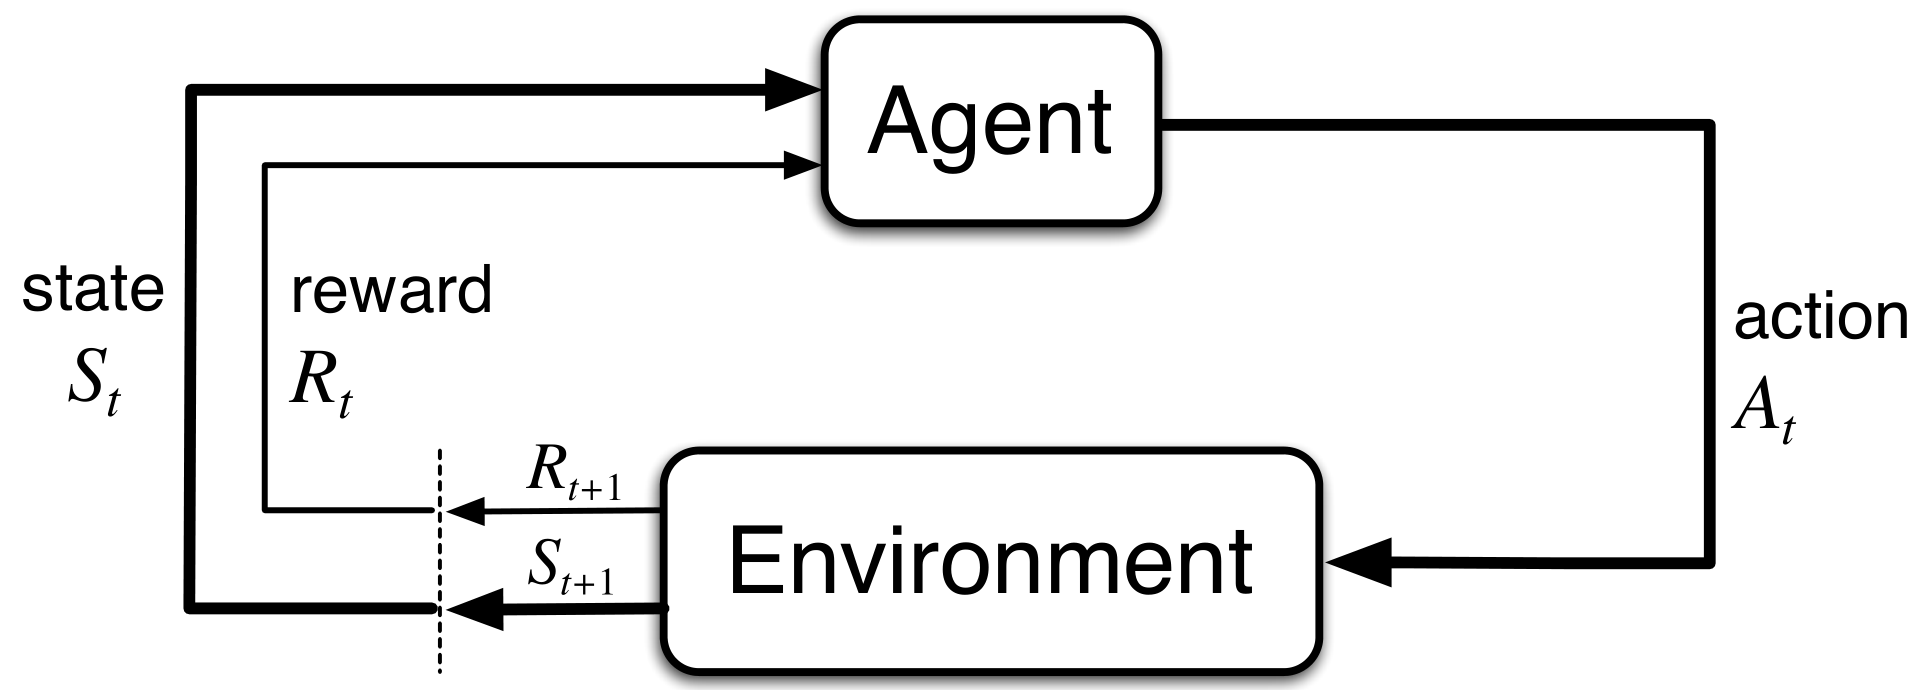
\includegraphics[width=.9\linewidth]{./fig/mdp_interaction.png}
\caption[Markov Decision Process]{The agent-environment interaction in a Markov decision process \cite{sutton18_reinf} \protect\footnotemark \label{agent-environment-interaction}}
\end{figure}
\footnotetext{\textbf{Figure 3.1} from "Reinforcement Learning: An Introduction" by Richard S. Sutton and Andew G. Barto is licencsed under CC BY-NC-ND 2.0 (https://creativecommons.org/licenses/by-nc-nd/2.0/)}

In RL the agent and the environment continuously interact with each other. The
agent takes actions that influence the environment, which in return presents
rewards to the agent. The agent's goal is to maximize rewards over time, trough
an optimal choice of actions. In each discrete timestep \(t\!=\!0,1,2,...,T\) the
RL agent interacts with the environment, which is perceived by the agent as a
representation, called \emph{state}, \(S_t \in \S\). Based on the state, the agents
selects an \emph{action}, \(A_t\in\A\), and receives a numerical \emph{reward} signal,
\(R_{t+1}\in\R\subset\Re\), in the next timestep. Actions influence immediate
rewards and successive states, and consequently also influence future rewards.
The agent has to continuously make a trade-off between immediate rewards and
delayed rewards to achieve its long-term goal.

The \emph{dynamics} of a MDP are defined by the probability that a state \(s'\in \S\)
and a reward \(r\in\R\) occurs, given the preceding state \(s\in\S\) and an action
\(a\in\A\). In \emph{finite} MDPs, the random variables \(\R_t\) and \(S_t\) have
well-defined probability density functions (PDF), which are solely dependent on
the previous state and action. Consequently, it is possible to define (\(\defeq\))
the \emph{dynamics} of the MDP as following:
\begin{equation} \label{eq-dynamics}
    p(s',r|s,a) \defeq \Pr{S_t=s',R_t=r|S_{t-1}=s,A_t=a},
\end{equation}
for all \(s',s\!\in\!\S\), \(r\!\in\!\R\) and \(a\!\in\!\A\). Note that each possible
value of the state \(\S_t\) depends only on the immediately preceding state
\(\S_{t-1}\). When a state includes all information of \emph{all} previous states, the
state possesses the so-called \emph{Markov property}. If not noted otherwise, the
Markov property is assumed throughout the whole chapter. The dynamics function
allows computing the \emph{state-transition probabilities}, another important
characteristic of an MDP, as following:
\begin{equation} \label{eq-state-transition}
    p(s'|s,a) \defeq \Pr{S_t\!=\!s'|S_{t-1}\!=\!s,A_t\!=\!a} = \sum_{r\in\R}{p(s', r|s, a)},
\end{equation}
for \(s',s\!\in\!\S\), \(r\!\in\!\R\) and \(a\!\in\!\A\).

The use of a \emph{reward signal} \(R_t\) to formalize the agent's goal is a unique
characteristic of RL. Each timestep the agent receives the rewards as a scalar
value \(\R_t\in\Re\). The sole purpose of the RL agent is to maximize the
long-term cumulative reward (as opposed to the immediate reward). The long-term
cumulative reward can also be expressed as the \emph{expected return} \(G_t\):
\begin{equation} \label{eq-expected-return}
\begin{split}
    G_t &\defeq R_{t+1} + \gamma R_{t+2} + \gamma R_{t+3} + \cdots \\
    &= \sum_{k=0}^{\infty}{\gamma^k R_{t+k+1}} \\
    &= R_{t+1} + \gamma G_{t+1},
\end{split}
\end{equation}
where \(\gamma\), \(0\leq\gamma\leq 1\), is the \emph{discount rate} parameter. The
discount rate determines how "myopic" the agent is. If \(\gamma\) approaches 0,
the agent is more concerned with maximizing immediate rewards. On the contrary,
when \(\gamma\!=\! 1\), the agent takes future rewards strongly into account, the
agent is "farsighted".

\subsubsection{Policies and Value Functions}
\label{sec:orgb60ed00}
An essential task of almost every RL agent is estimating \emph{value functions}.
These functions describe how "good" it is to be in a given state, or how "good"
it is to perform an action in a given state. More formally, they take a state
\(s\) or a state-action pair \(s,a\) as input and give the expected return \(G_t\) as
output. The expected return is dependent on the actions the agent will take in
the future. Consequently, value functions are formulated with respect to a
\emph{policy} \(\pi\). A policy is a mapping of states to actions; it describes the
probability that an agent performs a certain action, based on the current state.
More formally, the policy is defined as
\(\pi(a|s)\defeq\Pr{A_t\!=\!a|S_t\!=\!s}\), a PDF of all \(a\!\in\!\A\) for each
\(s\!\in\!\S\). The various RL approaches differ in how the policy is
updated, based on the agent's interaction with the environment.

As mentioned, there are value functions of states and value functions of
state-action pairs: The \emph{state-value function of policy} \(\pi\) is denoted as
\(\vpi(s)\) and is defined as the expected return when starting in \(s\) and
following policy \(\pi\):
\begin{equation} \label{eq-state-value}
    \vpi(s) \defeq \EE{\pi}{G_t|S_t\!=\!s}, \text{ for all } s\in\S
\end{equation}
The \emph{action-value function of policy} \(\pi\) is denoted as \(\qpi(s,a)\) and is
defined as the expected return when starting in \(s\), taking action \(a\) and
following policy \(\pi\) afterwards:
\begin{equation} \label{eq-action-value}
    \qpi(s,a) \defeq \EE{\pi}{G_t|S_t\!=\!s, A_t\!=\!a}, \text{ for all } a\in\A, s\in\S
\end{equation}
An \emph{optimal policy} \(\pi_*\) has a greater (or equal) expected return than all
other policies.  The \emph{optimal} state-value function and \emph{optimal} action-value
function are defined as follows:
\begin{equation}
    \vstar(s) \defeq \max_a \vpi(s), \text{ for all } s\in\S
\end{equation}
\begin{equation}
    \qstar(s,a) \defeq \max_a \qpi(s), \text{ for all } s\in\S, a\in\A
\end{equation}
The \emph{optimal} action-value function describes the expected return when taking
action \(a\) in state \(s\) following the optimal policy \(\pi_*\) afterwards.
Estimating \(\qstar\) to obtain an optimal policy is a substantial part of RL and
has been known as \emph{Q-learning} \cite{watkins92_q_learn}. Details can be found in
Chapter \ref{sec-td-learning}.

\subsubsection{Bellman Equations}
\label{sec:org098bee3}
A central characteristic of value functions is the recursive relationship
between the values. Similar to Equation (\ref{eq-expected-return}), current values are
related to expected values of successive states. This relationship is heavily
used in RL and has been formulated as \emph{Bellman equations}
\cite{bellman57_dynam_progr}. The Bellman equation for \(\vpi(s)\) is defined as
follows:
\begin{equation} \label{eq-bellman}
\begin{split}
    \vpi(s) &\defeq \EE{\pi}{G_t|S_t=s} \\
    &= \EE{\pi}{R_{t+1}+\gamma G_{t+1}|S_t\!=\!s} \\
    &= \sum_{a}{\pi(a|s)}\sum_{s',r}{p(s',r|s,a)}\bigg[r+\gamma\vpi(s')\bigg],
\end{split}
\end{equation}
where \(a\!\in\!\A\), \(s,s'\!\in\!\S\), \(r\!\in\!\R\).
In other words, the value of a state equals the immediate reward plus the
expected value of all possible successor states, weighted by their probability
of occurring. \(\vpi(s)\) is the only solution to its Bellman equation. The
Bellman equation of the optimal value function \(v_*\) is called the \emph{Bellman
optimality equation}:
\begin{equation} \label{eq-bellman-optimality}
\begin{split}
    \vstar(s) &= \max_{a\in\A(s)}q_{\pi_*}(s,a) \\
    &= \max_{a}\EE{\pi_*}{R_{t+1}+\gamma G_{t+1}|S_t\!=\!s, A_t\!=a} \\
    &= \max_{a}\EE{\pi_*}{R_{t+1}+\gamma \vstar(S_{t+1})|S_t\!=\!s, A_t\!=a} \\
    &= \max_{a}\sum_{s',r}{p(s',r|s,a)}\bigg[r+\gamma\vstar(s')\bigg]
\end{split}
\end{equation}
where \(a\!\in\!\A\), \(s,s'\!\in\!\S\), \(r\!\in\!\R\). In other words, the value of
a state under an optimal policy equals the expected return for the best action
from that state. Note that the Bellman optimality equation does not refer to a
specific policy, it has a unique solution independent from one. It can be seen
as an equation system, which can be solved when the dynamics of the environment
\(p\) are known. Similar Bellman equations to Equations (\ref{eq-bellman}) and
(\ref{eq-bellman-optimality}) can also be formed for \(\qpi(s,a)\) and
\(\qstar(s,a)\). Bellman equations form the basis for computing and approximating
value functions and were an important milestone in RL history. Most RL methods
are \emph{approximately} solving the Bellman optimality equation
(\ref{eq-bellman-optimality}), by using experienced state transitions instead of
expected transition probabilities. The most common methods will be explored in
the following chapters.

\subsubsection{Dynamic Programming}
\label{sec:org58db8b4}
\emph{Dynamic Programming} (DP) is a method to compute optimal policies, the primary
goal of every RL method. DP makes use of value functions to facilitate the
search for good policies. Once an optimal value function, (i.e., one that
satisfies the optimality Bellman equation) is found, optimal policies can be
easily obtained. Despite the limited utility of DP in real-world settings, it
provides the theoretical foundation for all other RL methods. In fact, all of
the RL methods try to achieve the same goal, but without the assumption of a
perfect model of the environment (e.g., known \emph{state-transition probabilities},
Eq. \ref{eq-state-transition}) and less computational effort. Because DP assumes
full knowledge of the environment, it is known as \emph{planning}, in which optimal
solutions are \emph{computed}. In \emph{control} problems (Chapter \ref{sec-td-learning}),
optimal solutions are \emph{learned} from an unknown environment.

The two most popular DP algorithms that compute optimal policies are called
\emph{policy iteration} and \emph{value iteration}. These methods perform "sweeps" through
the whole state set and update the estimated value of each state via an
\emph{expected update} operation. In policy iteration, a value function for a given
policy \(\vpi\) needs to be computed first (\emph{policy evaluation}). A sequence of
approximated value functions \(\{v_k\}\) are updated using the Bellman equation
for \(\vpi\) (Eq. \ref{eq-bellman}) until convergence to \(\vpi\) is achieved. After
computing the value function for a given policy, it is possible to modify the
policy and see if the value \(\vpi(s)\) for a given state increases (\emph{policy
improvement}). A way of doing this, is evaluating the action-value function
\(\qpi(s,a)\) by \emph{greedily} taking the best short-term action \(a\!\in\!A\) at a
given timestep. Alternating between these two steps monotonically improves the
policies and the value functions until they converge to the optimum. This
algorithm is called \emph{policy iteration}:
\begin{equation}
    \pi_0 \xrightarrow{\text{ E }} v_{\pi_0} \xrightarrow{\text{ I }}
    \pi_1 \xrightarrow{\text{ E }} v_{\pi_1} \xrightarrow{\text{ I }}
    \pi_2 \xrightarrow{\text{ E }} \hdots \xrightarrow{\text{ I }}
    \pi_* \xrightarrow{\text{ E }} \vstar,
\end{equation}
where \(\xrightarrow{\text{ E }}\) denotes a policy evaluation step,
\(\xrightarrow{\text{ I }}\) denotes a policy improvement step. \(\pi_*\) and
\(\vstar\) are the optimal policy and optimal value function, respectively. Note
that in each iteration of the policy iteration algorithm, a policy evaluation
has to be performed, which requires multiple sweeps through the state space. In
\emph{value iteration}, the policy evaluation step is stopped after one sweep. In
this case, the two previous steps can be combined into one single update step:
\begin{equation}
\begin{split}
    v_{k+1}(s) &\defeq \max_a \EE{}{R_{t+1}+\gamma \vstar(S_{t+1})|S_t\!=\!s, A_t\!=a} \\
    &= \max_{a}\sum_{s',r}{p(s',r|s,a)}\bigg[r+\gamma v_k(s')\bigg],
\end{split}
\end{equation}
where \(a\!\in\!\A\), \(s,s'\!\in\!\S\), \(r\!\in\!\R\). It can be shown, that for any
given \(v_0\), the sequence \({v_k}\) converges to the optimal value function
\({\vstar}\). In value iteration, the Bellman optimality equation
(\ref{eq-bellman-optimality}) is simply turned into an update rule. Both of the
algorithms can be effectively used to compute optimal values and value function
in finite MDPs with a perfect model of the environment.

\subsubsection{Temporal-Difference Learning \label{sec-td-learning}}
\label{sec:orgf185a0d}
The previous chapter dealt with solving a \emph{planning} problem, that is computing
an optimal solution (i.e., an optimal policy \(\pi_*\)) of an MDP when a perfect
model of the environment is known. In the following chapters, we will look at
\emph{model-free} prediction and \emph{model-free} control. As opposed to planning,
model-free methods learn from experience and require no prior knowledge of the
environment. Remarkably, these methods can still achieve optimal behavior.

The \emph{TD prediction problem} is concerned with estimating state-values \(\vpi\)
using past experiences of following a given policy \(\pi\). TD methods update an
estimate \(V\) of \(\vpi\) in every timestep. At time \(t\!+\!1\) they immediately
perform an update operation on \(V(S_t)\). Because of the step-by-step nature of
TD learning, it is categorized as \emph{online learning}. Also note that TD methods
perform update operations on value estimates based on other learned estimates, a
procedure called \emph{bootstrapping}. In simple TD prediction, the
value estimates \(V\) are updated as following:
\begin{equation} \label{eq-td-prediction}
    V(S_t) \leftarrow V(S_t) + \alpha\big[R_{t+1}+\gamma V(S_{t+1}) - V(S_t)\big],
\end{equation}
where \(\alpha\) is a constant \emph{step-size} parameter and \(\gamma\) is the
\emph{discount rate}. Here, the update of the state-value is performed using the
observed reward \(R_{t+1}\) and the estimated value \(V(S_{t+1})\).

When a model is not available, it is useful to estimate \emph{action-values}, instead
of \emph{state-values}. If the environment is completely known, it is possible for
the agent to look one step ahead and select the best action. Without that
knowledge, the value of each action in a given state needs to be estimated. The
latter constitutes a problem, since not every \emph{state-action} pair will be
visited when the agent follows a deterministic policy. A deterministic policy
\(\pi(a|s)\) returns exactly one action given the current state, hence the agent
will only observe returns for one of the actions. In order to evaluate the value
function for all \emph{state-action} pairs \(\qpi\), continuous \emph{exploration} needs to
be ensured. In other words, the agent has to explore state-action pairs which
are seemingly disadvantageous given the current policy. This dilemma is also
known as the \emph{exploration-exploitation} trade-off. One way to achieve exploration
is using \emph{stochastic} policies for the action selection. Stochastic policies
have a non-zero probability of selecting each action in each state. A typical
stochastic policy is the \emph{\(\epsilon\)-greedy policy}, which selects the action with
the highest estimated value, except for a probability \(\epsilon\), it selects an
action at random.
\begin{figure}[htbp]
\centering
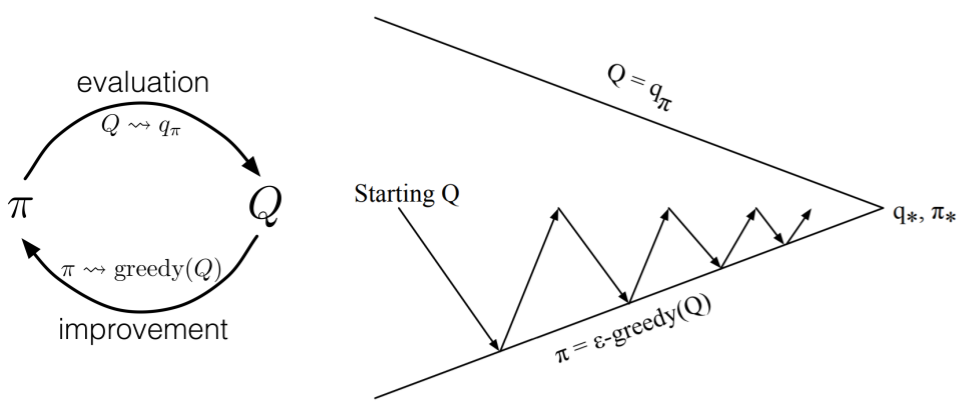
\includegraphics[width=.9\linewidth]{./fig/on-policy.png}
\caption[On-policy control with SARSA]{On-policy control with SARSA \cite{sutton18_reinf}. \protect\footnotemark \label{fig-sarsa}}
\end{figure}
\footnotetext{The in-text figure of \textbf{Chapter 5.3} from "Reinforcement Learning: An Introduction" by Richard S. Sutton and Andew G. Barto is licencsed under CC BY-NC-ND 2.0 (https://creativecommons.org/licenses/by-nc-nd/2.0/)}

There are two approaches to make use of stochastic policies to ensure all
actions are chosen infinitely often. On-policy methods improve the (stochastic)
decision policy, by continually estimating \(\qpi\) in regard to \(\pi\), while
simultaneously driving \(\pi\) towards \(\qpi\), e.g., with a \(\epsilon\)-greedy action
selection. Figure \ref{fig-sarsa} depicts this learning process. Off-policy
methods improve the deterministic decision policy, by using a second stochastic
policy to generate behavior. The first policy is becoming the optimal policy by
evaluating the exploratory behavior of the second policy. Off-policy approaches
are considered more powerful than on-policy approaches and have a variety of
additional use cases. On the other side, they often have a higher variance and
take more time to converge to an optimum.

A popular on-policy TD control method is SARSA, developed by
\textcite{rummery94_q}. In the prediction step, the action-value function
\(\qpi(s,a)\) of all actions and states has to be estimated for the current
policy \(\pi\). The estimation can be done similar to TD prediction of state
values (Eq. \ref{eq-td-prediction}). Instead of considering state transitions,
state-action transitions are considered in this case. The update rule is
constructed as follows:
\begin{equation} \label{eq-sarsa}
    Q(S_t, A_t) \leftarrow Q(S_t,A_t) + \alpha\big[R_{t+1}+\gamma Q(S_{t+1},A_{t+1}) - Q(S_t, A_t)\big]
\end{equation}
After every transition from a state \(S_t\), an update operation using the events
\((S_t, A_t, R_{t+1}, S_{t+1}, A_{t+1})\) is performed. This quintuple also
constituted the name SARSA. The on-policy control step of the algorithm is
straightforward, and uses a \(\epsilon\)-greedy policy improvement, as described in
the previous paragraph. It has been shown that SARSA converges to the optimal
policy \(\pi_*\) under the assumption of infinite visits to all state-action
pairs.

A breakthrough in RL has been achieved when \textcite{watkins92_q_learn} developed
the \emph{off-policy} TD control algorithm, called Q-learning. The update rule is
defined as follows:
\begin{equation} \label{eq-q-learning}
    Q(S_t, A_t) \leftarrow Q(S_t,A_t) + \alpha\big[R_{t+1}+\gamma\max_a Q(S_{t+1},a) - Q(S_t, A_t)\big]
\end{equation}
Here, the estimated action-values \(Q\) are updated towards the highest estimated
action-value of the next time step. In this way, \(Q\) directly approximates the
optimal action-value function \(q_*\), independently of the policy the agent
follows. Due to this simplification, Q-learning is a widely used model-free
method, and its convergence can be proved easily.

This chapter covered the most important RL methods. They work online,
learn from experience, and can be easily applied to real-world problems
with low computational effort. Moreover, the mathematical complexity of the
presented approaches is limited, and they can be easily implemented into
computer programs. Temporal-Difference learning is a \emph{tabular} method, Q-values
are stored and updated in a lookup table.

If the state and action spaces are continuous or the number of states and actions is
very large, a table representation is computational infeasible and the speed of
convergence is drastically reduced. In this case, a \emph{function approximator} can
replace the lookup table. The next chapter will briefly cover function approximation,
as well as other advancements in RL.
\subsubsection{Approximation Methods}
\label{sec:org85cc821}
All of the previous chapters covered tabular RL, which is the theoretical
foundation for all other methods. But in many real-world use cases the state
space is enormous and it is improbable to find an optimal value function with
tabular methods. Not only is the memory is problem to store such a large table,
but also the time needed to fill every entry with meaningful results.
Contrarily, \emph{function approximation} tries to find a function that approximates
the optimal value function as closely as possible, with limited computational
resources. The experience with a small subset of visited states is generalized
to approximate values of the whole state set. Function approximation has been
widely studied in supervised machine learning: Gradient methods, as well as
linear and non-linear models have shown good results for RL.

The approximated value of a state \(s\) is denoted as the parameterized
functional form \(\hat v(s,\w)\!\approx\!\vpi(s)\), given the weight vector
\(\w\!\in\!\Re^d\). Function approximation methods are approximating \(\vpi\) by
learning (i.e., adjusting) a weight vector \(\w\) from experience of following
the policy \(\pi\). By assumption, the dimensionality \(d\) of \(\w\) is much lower than
the number of states, which is the reason for the desired generalization effect:
Adjusting one weight affects the values of many states. On the other side, optimizing
an estimate for one state negatively affects the accuracy of the estimates for
other states. This effect motivates to specify a state distribution
\(\mu\), which represents the importance of the prediction error for each state.
The prediction error of a state is defined as the squared difference between the
predicted (i.e., approximated) value \(\hat v(s,\w)\) and the true value \(\vpi(s)\).
Consequently, the objective function of the supervised learning problem can be
defined as the \emph{Mean Squared Value Error} \(\MSVEm\), which weights
the prediction error with the state distribution \(\mu\):
\begin{equation}
    \MSVEm(\w) \defeq \sum_{s\in\S}{\mu(s)\bigg[\vpi(s)-\hat v(s,\w)\bigg]^2}, \text{ where } \w\in\Re^d
\end{equation}
Minimizing \(\MSVEm\) in respect to \(\hat v\) will yield in a value function that
helps achieving the primary goal of finding a better policy. Remember that \(\hat v\)
can take any form of linear or non-linear function of the features of a state.
In practice, deep artificial neural networks networks (ANNs) have shown great
success
\cite{mnih15_human_level_contr_throug_deep_reinf_learn,silver16_master_game_go_with_deep}.
A simplified feedforward ANN can be found in Figure \ref{fig-ann}, ANN have the advantage
that they can theoretically approximate any continuous function by adjusting the
connection weights of the network \(\w\in\Re^{d\times d}\).
\begin{figure}[htbp]
\centering
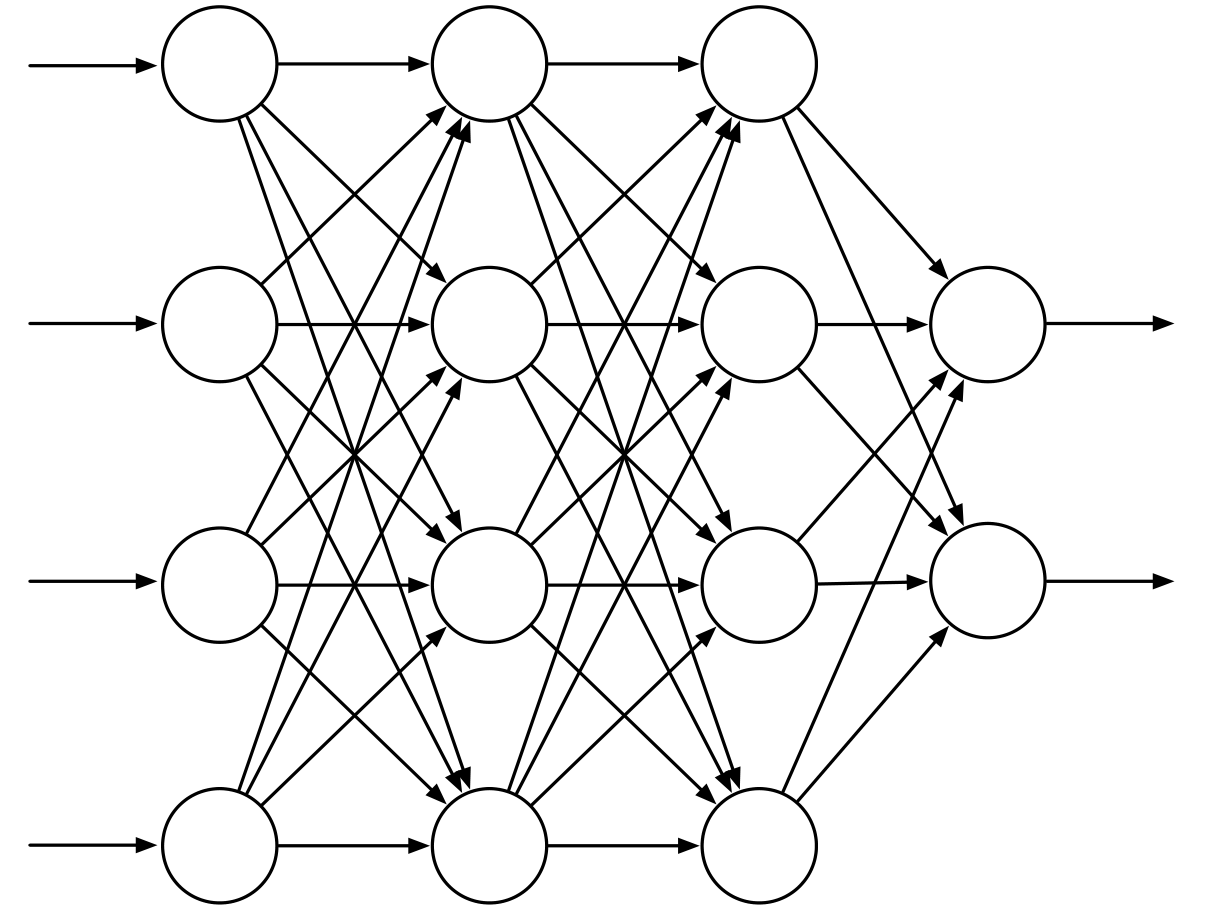
\includegraphics[width=.9\linewidth]{./fig/ann.png}
\caption[Artificial Neural Network]{A sample ANN consisting of four input nodes, two fully connected hidden layers and two output nodes \cite{sutton18_reinf}. \protect\footnotemark \label{fig-ann}}
\end{figure}
\footnotetext{\textbf{Figure 9.14} from "Reinforcement Learning: An Introduction" by Richard S. Sutton and Andew G. Barto is licencsed under CC BY-NC-ND 2.0 (https://creativecommons.org/licenses/by-nc-nd/2.0/)}

\section{Empirical Setting / Data (10\%)}
\label{sec:orgea38fcd}
\subsection{Carsharing Fleets of Electric Vehicles}
\label{sec:org7ca4b1e}
\subsubsection{Raw Data}
\label{sec:org4ccd781}
The dataset consists of 500 EVs in Stuttgart. As displayed in Table
\ref{car2go-sample-data}, the data contain spatio-temporal attributes, such as
timestamp, coordinates, and address of the EVs. Additionally, status attributes
of the interior and exterior are given, the relative state of charge and
information whether the EV is plugged into one of the 200 charging stations in
Stuttgart.

\begin{longtable}{l|ccccc}
\caption{Raw Car2Go Trip Data from Stuttgart \label{car2go-sample-data}}
\\
\hline
\hline
Number Plate & Latitude & Longitude & Street & Zip Code & Engine Type\\
\hline
\endfirsthead
\multicolumn{6}{l}{Continued from previous page} \\
\hline

Number Plate & Latitude & Longitude & Street & Zip Code & Engine Type \\

\hline
\endhead
\hline\multicolumn{6}{r}{Continued on next page} \\
\endfoot
\endlastfoot
\hline
S-GO2471 & 9.19121 & 48.68895 & Parkplatz Flughafen & 70692 & electric\\
S-GO2471 & 9.15922 & 48.78848 & Salzmannweg 3 & 70192 & electric\\
S-GO2471 & 9.17496 & 48.74928 & Felix-Dahn-Str.45 & 70597 & electric\\
S-GO2471 & 9.17496 & 48.74928 & Felix-Dahn-Str.45 & 70597 & electric\\
S-GO2471 & 9.17496 & 48.74928 & Felix-Dahn-Str.45 & 70597 & electric\\
\hline
Number Plate & Interior & Exterior & Timestamp & Charging & State of Charge\\
\hline
S-GO2471 & good & good & 22.12.2017 20:10 & no & 94\\
S-GO2471 & good & good & 24.12.2017 23:05 & no & 72\\
S-GO2471 & good & good & 26.12.2017 00:40 & yes & 81\\
S-GO2471 & good & good & 26.12.2017 00:45 & yes & 83\\
S-GO2471 & good & good & 26.12.2017 00:50 & yes & 84\\
\hline
\hline
\end{longtable}
\subsubsection{Preprocessing Steps}
\label{sec:org92c82a7}
\subsection{Electricity Markets Data}
\label{sec:org5fc2fc8}
\subsubsection{Secondary Operating Reserve Market}
\label{sec:org84d0489}
\subsubsection{Intraday Continuous Spot Market}
\label{sec:orga23153c}

\section{Model: FleetRL (20\%)}
\label{sec:org423ec2c}
\subsection{Information Assumptions}
\label{sec:orge729062}
\subsection{Mobility Demand \& Clearing Price Prediction}
\label{sec:org6d1942e}
\subsection{Reinforcement Learning Approach}
\label{sec:org92ccc15}
\subsection{Bidding Strategy}
\label{sec:orgf7655e6}
\subsection{Dispatch Heuristic / Algorithm}
\label{sec:org0ca312d}

\section{Evaluation (30\%)}
\label{sec:orgcb6eaf5}
\subsection{Event-based Simulation}
\label{sec:orge140c9c}
\subsection{Benchmark: Ad-hoc Strategies}
\label{sec:org660ad9f}
\subsection{FleetRL}
\label{sec:org904baa6}
\subsection{Sensitivity Analysis: Prediction Accuracy}
\label{sec:org2b38dc9}
\subsection{Sensitivity Analysis: Infrastructure Changes}
\label{sec:orgfb6bf1d}
\subsection{Sensitivity Analysis: Bidding Strategy}
\label{sec:orgbe55309}
\section{Discussion (5\%)}
\label{sec:orge6e3c66}
\subsection{Generalizability}
\label{sec:org8d02784}
\subsection{Future Electricity Landscape}
\label{sec:orgaa15039}
\subsection{Limitations}
\label{sec:orgba65e1f}
\section{Conclusion (5\%)}
\label{sec:orgb3a1c94}
\subsection{Contribution}
\label{sec:org72e8b7c}
\subsection{Future Research}
\label{sec:org5e88949}


\clearpage
\bibliography{bibliography/references}
\bibliographystyle{apacite}
\end{document}
